% !TeX program = xelatex
% 概率论与数理统计 第1--3章复习课
% 编译：xelatex probability_review.tex（连续两次）
% 学生版：取消下一行注释，隐藏六道章后练习的答案页。
% \def\StudentVersion{1}
\documentclass[aspectratio=169,10pt]{beamer}
\usepackage{xeCJK}
\usepackage{amsmath,amssymb,mathtools,booktabs,array}
\usepackage{tikz}
\usetikzlibrary{arrows.meta,positioning,calc,patterns}
\usepackage{appendixnumberbeamer}
\IfFontExistsTF{Noto Sans CJK SC}{
  \setCJKmainfont{Noto Sans CJK SC}\setCJKsansfont{Noto Sans CJK SC}
}{\IfFontExistsTF{Microsoft YaHei}{
  \setCJKmainfont{Microsoft YaHei}\setCJKsansfont{Microsoft YaHei}
}{\setCJKmainfont{FandolHei-Regular}[BoldFont=FandolHei-Bold]
  \setCJKsansfont{FandolHei-Regular}[BoldFont=FandolHei-Bold]}}
\setsansfont{Latin Modern Sans}
\setmainfont{Latin Modern Roman}
\usefonttheme{professionalfonts}
\definecolor{Navy}{HTML}{16324F}
\definecolor{Teal}{HTML}{087E8B}
\definecolor{Amber}{HTML}{B96820}
\definecolor{Ink}{HTML}{233747}
\definecolor{Muted}{HTML}{60717E}
\definecolor{Paper}{HTML}{FCFCF8}
\definecolor{PaleTeal}{HTML}{EAF5F4}
\definecolor{PaleAmber}{HTML}{FBF0E4}
\setbeamercolor{background canvas}{bg=Paper}
\setbeamercolor{normal text}{fg=Ink}
\setbeamercolor{structure}{fg=Teal}
\setbeamercolor{frametitle}{fg=Navy}
\setbeamercolor{title}{fg=Navy}
\setbeamercolor{subtitle}{fg=Teal}
\setbeamercolor{block title}{fg=Teal,bg=PaleTeal}
\setbeamercolor{block body}{fg=Ink,bg=PaleTeal!55!Paper}
\setbeamercolor{block title alerted}{fg=Amber,bg=PaleAmber}
\setbeamercolor{block body alerted}{fg=Ink,bg=PaleAmber!55!Paper}
\setbeamerfont{title}{size=\LARGE,series=\bfseries}
\setbeamerfont{subtitle}{size=\large}
\setbeamerfont{frametitle}{size=\Large,series=\bfseries}
\setbeamerfont{block title}{size=\normalsize,series=\bfseries}
\setbeamerfont{footline}{size=\tiny}
\setbeamertemplate{navigation symbols}{}
\setbeamertemplate{itemize item}{\color{Teal}\small$\blacktriangleright$}
\setbeamertemplate{itemize subitem}{\color{Teal}$\bullet$}
\setbeamersize{text margin left=7.5mm,text margin right=7.5mm}
\setbeamertemplate{frametitle}{
  \vspace{2mm}\insertframetitle\par\vspace{1mm}
  {\color{Teal}\rule{\linewidth}{0.6pt}}\vspace{-1mm}}
\setbeamertemplate{footline}{
  \leavevmode\hbox{\hspace{7.5mm}
  \begin{beamercolorbox}[wd=.74\paperwidth,ht=2.6ex,dp=1.4ex]{normal text}
  \color{Muted}概率论与数理统计\quad /\quad \insertsectionhead
  \end{beamercolorbox}
  \begin{beamercolorbox}[wd=.15\paperwidth,ht=2.6ex,dp=1.4ex,right]{normal text}
  \color{Teal}\insertframenumber\, /\,\inserttotalframenumber
  \end{beamercolorbox}}}
\setlength{\parskip}{1.5pt}
\let\reviewnormalsize\normalsize
\renewcommand{\normalsize}{\reviewnormalsize
  \setlength{\abovedisplayskip}{5pt plus 1pt minus 1pt}
  \setlength{\belowdisplayskip}{5pt plus 1pt minus 1pt}
  \setlength{\abovedisplayshortskip}{3pt plus 1pt}
  \setlength{\belowdisplayshortskip}{3pt plus 1pt}}
\newcommand{\dd}{\,\mathrm{d}}
\newcommand{\R}{\mathbb{R}}
\newcommand{\ind}{\mathbf{1}}
\DeclareMathOperator{\Exp}{Exp}
\DeclareMathOperator{\Pois}{Pois}
\newcommand{\source}[1]{\vfill{\color{Muted}\fontsize{6.5}{8}\selectfont 资料：#1\par}}
\newcommand{\key}[1]{\begin{block}{要点}#1\end{block}}
\newcommand{\warn}[1]{\begin{alertblock}{易错提醒}#1\end{alertblock}}
\newif\ifshowanswers
\ifdefined\StudentVersion\showanswersfalse\else\showanswerstrue\fi
\NewDocumentEnvironment{answerframe}{m +b}{%
  \ifshowanswers\begin{frame}[t]{#1}#2\end{frame}\fi}{}
\title{概率论与数理统计}
\subtitle{第1--3章复习串讲\quad 事件 → 分布 → 联合分布}
\author{知识主线 · 重点方法 · 章后练习}
\date{}
\begin{document}
\section{课程导览}

\begin{frame}[plain]
\vspace{6mm}
{\color{Teal}\small REVIEW\quad /\quad CHAPTERS 01--03}\par
\vspace{4mm}
{\color{Navy}\LARGE\bfseries 概率论与数理统计}\par
\vspace{3mm}
{\color{Navy}\Large 第1--3章复习串讲}\par
\vspace{5mm}
{\large 随机事件\quad$\longrightarrow$\quad 一维随机变量\quad$\longrightarrow$\quad 二维随机变量}
\vspace{5mm}
\begin{tikzpicture}
\foreach \x/\n/\t in {0/01/事件与概率,4.8/02/随机变量及其分布,9.6/03/二维随机变量}{
  \node[anchor=west,fill=PaleTeal,rounded corners=2pt,minimum width=4.3cm,
  minimum height=1cm,text width=4cm,inner sep=3mm] at (\x,0)
  {\color{Teal}\bfseries\n\quad\color{Ink}\t};}
\end{tikzpicture}
\vfill
{\color{Muted}\small 依据所提供笔记与2023年六份自测题、补充题整理}
\note{开场先问：遇到一道题，如何判断应当用事件公式、分布函数，还是联合分布？本课围绕这个判断串联三章。}
\end{frame}

\begin{frame}[t]{三章总览：研究对象与核心问题}
\renewcommand{\arraystretch}{1.5}
\begin{tabular}{p{2.6cm}p{5.1cm}p{5.3cm}}
\toprule
\textbf{章节} & \textbf{主要内容} & \textbf{要会解决的问题}\\\midrule
\textbf{第一章}\par 概率论的基本概念 & 样本空间、事件运算、概率模型、条件概率、全概率、贝叶斯、独立性 & 把文字翻译成事件，选择公式并算出概率\\
\textbf{第二章}\par 随机变量及其分布 & 分布律、分布函数、概率密度、常见分布、随机变量函数的分布 & 从分布描述求概率，从$X$的分布求$g(X)$的分布\\
\textbf{第三章}\par 二维随机变量 & 联合、边缘与条件分布、独立性、和差与最值的分布 & 从联合分布提取信息，求$g(X,Y)$的分布\\\bottomrule
\end{tabular}
\source{笔记，第1--22页（第22页第四章开头不纳入本课范围）。}
\end{frame}

\begin{frame}[t]{三章共用的解题流程}
\begin{enumerate}
\item \textbf{定义对象：}事件是什么？随机变量记录什么？
\item \textbf{确定范围：}样本空间、可能取值、密度的非零区域。
\item \textbf{翻译目标：}把“至少”“已知”“最大值”等写成数学事件。
\item \textbf{选择工具：}计数、条件概率、求和、积分、分布函数法。
\item \textbf{检查结果：}非负、总概率为1、边界正确、适用条件齐全。
\end{enumerate}
\key{贯穿全课的两个问题：\quad\textbf{概率加在哪些点上？积分积在哪个区域上？}}
\source{根据三章笔记与六份习题归纳。}
\end{frame}

\section{第一章\quad 概率论的基本概念}
\begin{frame}[t]{第一章概览：先描述事件，再计算概率}
\begin{columns}[T]
\column{.48\textwidth}
\begin{block}{知识结构}
随机试验与样本空间$\Omega$\\[2mm]
$\downarrow$\quad 事件的关系与运算\\[2mm]
概率的公理与性质\\[2mm]
$\downarrow$\quad 条件概率与乘法公式\\[2mm]
全概率、贝叶斯与独立性
\end{block}
\column{.47\textwidth}
\textbf{本章重点}
\begin{itemize}
\item “至少一个”常用对立事件。
\item “已知”意味着条件概率。
\item “分来源”用全概率公式。
\item “由结果反推来源”用贝叶斯公式。
\item 分清互斥、对立、独立。
\end{itemize}
\end{columns}
{\small 随机试验：可重复、可能结果已知、单次结果不确定。\\
频率是观测比例，可用来估计概率；一次抽样的比例不等于总体真实概率。}
\source{笔记，第1--4页；自测题-1与补充题-1。}
\end{frame}

\begin{frame}[t]{事件运算：先把中文翻译准确}
设$A_i=\{\text{第$i$次命中}\}$，$i=1,2,3$。
\renewcommand{\arraystretch}{1.4}
\begin{center}
\begin{tabular}{ll}
\toprule
至少命中一次 & $A_1\cup A_2\cup A_3=\overline{\bar A_1\bar A_2\bar A_3}$\\
三次全部命中 & $A_1A_2A_3$\\
至少一次未命中 & $\overline{A_1A_2A_3}=\bar A_1\cup\bar A_2\cup\bar A_3$\\
恰好一次命中 & $A_1\bar A_2\bar A_3\cup\bar A_1A_2\bar A_3\cup\bar A_1\bar A_2A_3$\\
发生$A$但不发生$B$ & $A\setminus B=A\bar B$\\\bottomrule
\end{tabular}
\end{center}
\key{德摩根律：$\overline{A\cup B}=\bar A\bar B$，\quad$\overline{AB}=\bar A\cup\bar B$。}
\source{笔记，第1--2页；自测题-1，一、3及二、1；补充题-1，二。}
\end{frame}

\begin{frame}[t]{概率的公理与高频公式}
\textbf{三条公理：}非负性$P(A)\ge0$；规范性$P(\Omega)=1$；可列可加性。
若$A_1,A_2,\ldots$两两互斥，则
\[
P\left(\bigcup_{i=1}^{\infty}A_i\right)=\sum_{i=1}^{\infty}P(A_i).
\]
\begin{columns}[T]
\column{.48\textwidth}
\begin{block}{从公理得到的计算公式}
\vspace{-2mm}
\begin{align*}
P(\bar A)&=1-P(A),\\
P(A\setminus B)&=P(A)-P(AB),\\
P(A\cup B)&=P(A)+P(B)-P(AB).
\end{align*}
\end{block}
\column{.47\textwidth}
\textbf{交事件概率的取值范围}
\[
\max\{0,P(A)+P(B)-1\}\le P(AB)
\]
\[
P(AB)\le\min\{P(A),P(B)\}.
\]
用它快速检查数据是否自洽。
\end{columns}
\source{笔记，第2页；补充题-1，三、3。}
\end{frame}

\begin{frame}[t]{古典概型与几何概型：关键是等可能性}
\begin{columns}[T]
\column{.48\textwidth}
\begin{block}{古典概型：有限且等可能}
\[
P(A)=\frac{\#A}{\#\Omega}.
\]
计数前先统一口径：
\begin{itemize}
\item 是否区分先后顺序？
\item 是否放回？对象是否可区分？
\end{itemize}
\end{block}
\textbf{例：}三个不同的球独立等可能放入四个盒子，恰占三个盒子的概率
\[
\frac{4\times3\times2}{4^3}=\frac38.
\]
\column{.47\textwidth}
\begin{block}{几何概型：在区域上均匀取点}
\[
P(A)=\frac{m(A)}{m(\Omega)}.
\]
$m$表示长度、面积或体积。
\end{block}
\warn{“有无穷多个结果”不足以推出几何概型；必须说明取点均匀。}
\end{columns}
\source{笔记，第3页；自测题-1，一、4。}
\end{frame}

\begin{frame}[t]{条件概率与乘法公式：条件改变了参照范围}
当$P(B)>0$时，
\[
\boxed{P(A\mid B)=\frac{P(AB)}{P(B)}}
\qquad\Longleftrightarrow\qquad
\boxed{P(AB)=P(B)P(A\mid B)}.
\]
\begin{block}{多步试验：按发生顺序逐步相乘}
\[
P(ABC)=P(A)P(B\mid A)P(C\mid AB).
\]
每一步都要更新条件；无放回抽样通常不能直接相乘边缘概率。
\end{block}
\textbf{例：}10件产品有4件次品，依次无放回取2件，两件均为次品的概率
\[
\frac4{10}\cdot\frac3{9}=\frac{\binom42}{\binom{10}2}=\frac2{15}.
\]
\source{笔记，第3页；补充题-1，四、4的抽样情境。}
\end{frame}

\begin{frame}[t]{全概率与贝叶斯：同一张“来源—结果”图}
设$B_1,\ldots,B_n$两两互斥，$\bigcup_iB_i=\Omega$，且$P(B_i)>0$。
\begin{columns}[T]
\column{.36\textwidth}
\begin{tikzpicture}[>=Stealth,node distance=11mm,every node/.style={font=\small}]
\node (s) at (0,0) {$\Omega$};
\node (b1) at (1.6,1) {$B_1$};\node (b2) at (1.6,0) {$B_2$};\node (bn) at (1.6,-1) {$B_n$};
\node (a) at (3.2,0) {$A$};
\draw[->,Teal] (s)--(b1);\draw[->,Teal] (s)--(b2);\draw[->,Teal] (s)--(bn);
\draw[->,Teal] (b1)--(a);\draw[->,Teal] (b2)--(a);\draw[->,Teal] (bn)--(a);
\node[Muted] at (1.6,-1.7) {各路径贡献相加};
\end{tikzpicture}
\column{.61\textwidth}
\textbf{由来源求结果：全概率公式}
\[
P(A)=\sum_{i=1}^nP(B_i)P(A\mid B_i).
\]
\textbf{已知结果，反推来源：贝叶斯公式}
\[
P(B_k\mid A)=\frac{P(B_k)P(A\mid B_k)}{\sum_iP(B_i)P(A\mid B_i)},\quad P(A)>0.
\]
\end{columns}
\key{先定义划分；分母把所有可能来源的贡献都加上。}
\source{笔记，第4页；自测题-1，四、4--6；补充题-1，四、10--12。}
\end{frame}

\begin{frame}[t]{笔记例题：检测阳性后，患病概率有多大？}
设$D=\{\text{患病}\}$，$T=\{\text{检测阳性}\}$。已知
\[
P(D)=0.001,\quad P(T\mid D)=0.99,\quad P(\bar T\mid\bar D)=0.98.
\]
\begin{align*}
P(T)&=0.001\times0.99+0.999\times0.02=0.02097,\\[1mm]
P(D\mid T)&=\frac{0.001\times0.99}{0.02097}\approx\boxed{4.72\%}.
\end{align*}
\begin{block}{用10万人理解贝叶斯分母}
约100人患病，其中99人阳性；约99\,900人未患病，其中1\,998人假阳性。
阳性人群中患病者占$99/(99+1998)$。
\end{block}
\source{笔记，第4页检测例题；数值重新计算。}
\note{强调0.98是特异度，假阳性率是0.02。让学生指出P(T|D)与P(D|T)的条件分别是什么。}
\end{frame}

\begin{frame}[t]{独立、互斥、对立：三个不同概念}
\renewcommand{\arraystretch}{1.5}
\begin{tabular}{p{1.8cm}p{5.2cm}p{6cm}}
\toprule
关系 & 定义 & 结论\\\midrule
互斥 & $AB=\varnothing$ & $P(AB)=0$\\
对立 & $B=\bar A$ & 互斥且并集为$\Omega$\\
独立 & $P(AB)=P(A)P(B)$ & 若$P(B)>0$，则$P(A\mid B)=P(A)$\\\bottomrule
\end{tabular}
\vspace{3mm}
\begin{itemize}
\item 当$P(A),P(B)>0$时，互斥事件\textbf{不独立}。
\item $A,B$独立，则$A,\bar B$、$\bar A,B$、$\bar A,\bar B$均独立。
\item 一般情况下，$P(A)=0$不等于$A=\varnothing$。
\end{itemize}
\source{笔记，第2、4页；自测题-1，三、2--6及10。}
\end{frame}

\begin{frame}[t]{两两独立不能替代相互独立}
三事件相互独立，必须同时满足
\[
\begin{gathered}
P(AB)=P(A)P(B),\quad P(AC)=P(A)P(C),\quad P(BC)=P(B)P(C),\\
P(ABC)=P(A)P(B)P(C).
\end{gathered}
\]
\begin{block}{反例：独立抛两次均匀硬币}
$A=\{\text{第一次正面}\}$，$B=\{\text{第二次正面}\}$，$C=\{\text{恰好一次正面}\}$。
\[
P(A)=P(B)=P(C)=\frac12,\qquad P(AB)=P(AC)=P(BC)=\frac14.
\]
但$ABC=\varnothing$，所以$P(ABC)=0\ne\frac18$。
\end{block}
\key{“分别与两个事件独立”也不能直接推出“与它们的并独立”。}
\source{笔记，第4页；补充题-1，三、8；自测题-1，三、7--9。}
\end{frame}

\begin{frame}[t]{第一章收束：看到题目关键词，选对公式}
\renewcommand{\arraystretch}{1.45}
\begin{tabular}{p{3.7cm}p{8.9cm}}
\toprule
\textbf{题目结构} & \textbf{优先考虑}\\\midrule
至少一个、至少一次 & 对立事件：$1-P(\text{一个也没有})$\\
恰好若干个 & 互斥分类；满足独立同分布时可用二项模型\\
已知某事件发生 & $P(A\mid B)=P(AB)/P(B)$\\
分批次、分地区、分类型 & 建立完备划分，使用全概率公式\\
已知结果，求来自哪一类 & 贝叶斯公式\\
多个事件相乘 & 先检查独立性；否则使用条件概率连乘\\\bottomrule
\end{tabular}
\source{依据自测题-1、补充题-1归纳。}
\end{frame}

\begin{frame}[t]{第一章练习1：已知“至少一件次品”}
\begin{block}{题目\quad 建议3分钟}
10件产品中有4件次品、6件合格品。从中随机无放回取2件。

已知取出的2件中\textbf{至少有1件次品}，求另一件为合格品的概率。
\end{block}
\vspace{3mm}
\textbf{思考顺序}
\begin{enumerate}
\item 条件事件$B$是什么？
\item 在条件$B$下，目标对应哪个事件？
\item 分母应当统计哪几类取法？
\end{enumerate}
\source{改写自补充题-1，四、4，第3页；将原题“有一件”明确为“至少一件”。}
\end{frame}

\begin{answerframe}{第一章练习1答案：条件下的样本空间}
设$B=\{\text{至少一件次品}\}$，$A=\{\text{恰一件次品、一件合格品}\}$。
由于$A\subseteq B$，
\[
P(A\mid B)=\frac{P(A)}{P(B)}
=\frac{\binom41\binom61}{\binom41\binom61+\binom42}
=\frac{24}{24+6}=\boxed{\frac45}.
\]
\begin{block}{也可以从对立事件计算分母}
\[
P(B)=1-\frac{\binom62}{\binom{10}2}=\frac{30}{45},\qquad P(A)=\frac{24}{45}.
\]
\end{block}
\warn{“至少有一件次品”包括“两件均为次品”；分母不能只保留混合取法。}
\source{补充题-1，四、4，第3页。}
\end{answerframe}

\begin{frame}[t]{第一章练习2：连取白球后的来源判断}
\begin{block}{题目\quad 建议4分钟}
甲袋有2白4黑，乙袋有4白2黑。先掷一枚均匀硬币，正面选甲袋，反面选乙袋。

选袋后，在同一袋内连续取球$n$次，\textbf{每次取后放回}。
已知$n$次全部取到白球，求所选袋为甲袋的概率（$n\ge1$）。
\end{block}
\vspace{2mm}
\textbf{思考顺序}
\begin{enumerate}
\item 哪两个事件构成样本空间的划分？
\item 在选袋条件下，$n$次全部为白球的概率分别是多少？
\item 当$n$增大，答案应该上升还是下降？
\end{enumerate}
\source{自测题-1，四、5，第4页。}
\end{frame}

\begin{answerframe}{第一章练习2答案：先算似然，再更新来源概率}
设$H=\{\text{选甲袋}\}$，$W_n=\{n\text{次全白}\}$。则
\[
P(H)=P(\bar H)=\frac12,\qquad
P(W_n\mid H)=\left(\frac13\right)^n,\qquad
P(W_n\mid\bar H)=\left(\frac23\right)^n.
\]
由贝叶斯公式，
\[
P(H\mid W_n)=\frac{\frac12(\frac13)^n}{\frac12(\frac13)^n+\frac12(\frac23)^n}
=\boxed{\frac1{1+2^n}}.
\]
\key{$n=1$时为$1/3$；$n$越大，选乙袋的证据越强，甲袋的后验概率趋于0。}
\source{自测题-1，四、5，第4页。}
\note{取后放回保证在选定袋的条件下各次独立；未给定选袋信息时，不可把单次无条件白球概率的n次方当作全白概率。}
\end{answerframe}

\section{第二章\quad 随机变量及其分布}

\begin{frame}[t]{第二章概览：用分布完整描述一个随机变量}
\begin{columns}[T]
\column{.48\textwidth}
\begin{block}{三种分布描述}
\textbf{通用描述：}分布函数$F_X(x)$。\\[3mm]
\textbf{离散型：}分布律$p_k=P(X=x_k)$。\\[3mm]
\textbf{连续型：}概率密度$f_X(x)$。
\end{block}
\column{.47\textwidth}
\textbf{本章重点}
\begin{itemize}
\item 规范性：概率之和或积分为1。
\item 分布函数的右连续与跳跃。
\item 常见分布的识别及概率计算。
\item 分布函数法求$Y=g(X)$的分布。
\item 连续变量变换后也可能有点概率。
\end{itemize}
\end{columns}
\source{笔记，第5--13页；自测题-2与补充题-2。}
\end{frame}

\begin{frame}[t]{随机变量与分布律：结果数值化，概率不丢失}
随机变量是定义在样本空间上的实值函数$X:\Omega\to\R$。
\begin{block}{离散型分布律}
\[
P(X=x_k)=p_k,\qquad p_k\ge0,\qquad\sum_kp_k=1.
\]
求事件概率：$\displaystyle P(X\in A)=\sum_{x_k\in A}p_k$。
\end{block}
\textbf{例：}若$P(X=k)=c(2/3)^k$，$k=1,2,\ldots$，则
\[
1=c\sum_{k=1}^{\infty}\left(\frac23\right)^k
=c\frac{2/3}{1-2/3}=2c\quad\Longrightarrow\quad\boxed{c=\frac12}.
\]
\source{笔记，第5--6页；补充题-2，一、4，第1页。}
\end{frame}

\begin{frame}[t]{分布函数：所有类型的随机变量都适用}
\[
\boxed{F_X(x)=P(X\le x)},\qquad x\in\R.
\]
\begin{columns}[T]
\column{.48\textwidth}
\textbf{判断一个函数是否为分布函数}
\begin{enumerate}
\item 单调不减。
\item $F(-\infty)=0$，$F(+\infty)=1$。
\item 右连续：$F(x+)=F(x)$。
\end{enumerate}
\column{.47\textwidth}
\begin{block}{跳跃量就是点概率}
记$F(a-)=\lim_{x\uparrow a}F(x)$，则
\[
\boxed{P(X=a)=F(a)-F(a-)}.
\]
有跳跃的分布函数可以是离散型，也可以是混合型。
\end{block}
\end{columns}
\source{笔记，第7--8页；自测题-2，一、1及5，二、1。}
\end{frame}

\begin{frame}[t]{端点开闭：先写事件，再代分布函数}
对任意$a<b$，
\renewcommand{\arraystretch}{1.45}
\begin{center}
\begin{tabular}{ll@{\hspace{1cm}}ll}
\toprule
$P(X<a)$ & $F(a-)$ & $P(X\le a)$ & $F(a)$\\
$P(X>a)$ & $1-F(a)$ & $P(X\ge a)$ & $1-F(a-)$\\\midrule
$P(a<X\le b)$ & $F(b)-F(a)$ & $P(a\le X\le b)$ & $F(b)-F(a-)$\\
$P(a<X<b)$ & $F(b-)-F(a)$ & $P(a\le X<b)$ & $F(b-)-F(a-)$\\\bottomrule
\end{tabular}
\end{center}
\begin{block}{例：$P(X=-1)=P(X=1)=1/2$}
$P(-1<X\le1)=1/2$，而$P(-1\le X\le1)=1$。
\end{block}
\warn{只有端点的点概率为0时，才可以忽略该端点的开闭；连续型变量满足这一条件。}
\source{笔记，第7--8页；自测题-2，一、3及5。}
\end{frame}

\begin{frame}[t]{概率密度与分布函数：积分得到概率}
连续型随机变量有密度$f_X$，满足
\[
f_X(x)\ge0,\qquad\int_{-\infty}^{+\infty}f_X(x)\dd x=1,
\qquad F_X(x)=\int_{-\infty}^{x}f_X(t)\dd t.
\]
\begin{columns}[T]
\column{.48\textwidth}
\begin{block}{例：$f(x)=2x\ind_{(0,1)}(x)$}
\[
F(x)=\begin{cases}0,&x<0,\\x^2,&0\le x<1,\\1,&x\ge1.\end{cases}
\]
\end{block}
\column{.47\textwidth}
\[
P(X\le\tfrac12)=\int_0^{1/2}2x\dd x=\frac14.
\]
\[
P(X=\tfrac12)=0.
\]
密度可以大于1，也不必连续。\\
在$f$连续处，$F'(x)=f(x)$。
\end{columns}
{\small 记号$\ind_D$表示指示函数：在$D$内取1，在$D$外取0。}
\source{笔记，第8--9页；补充题-2，三、2--3，第3--4页。}
\end{frame}

\begin{frame}[t]{常见离散分布：先识别试验结构}
\small
\renewcommand{\arraystretch}{1.65}
\begin{tabular}{p{2.5cm}p{6.2cm}p{4.2cm}}
\toprule
分布 & 分布律 & 识别线索\\\midrule
0--1分布 & $P(X=1)=p,\ P(X=0)=1-p$ & 一次试验，成功或失败\\
二项分布$B(n,p)$ & $P(X=k)=\binom nkp^k(1-p)^{n-k}$\par $k=0,1,\ldots,n$ & $n$次独立、成功概率相同；数成功次数\\
泊松分布$\Pois(\lambda)$ & $P(X=k)=e^{-\lambda}\lambda^k/k!$\par $k=0,1,\ldots$，$\lambda>0$ & 单位时间或区域内的事件次数\\\bottomrule
\end{tabular}
\normalsize
有限$m$个等可能取值构成离散均匀分布，每点概率为$1/m$。
\key{若$X\sim B(n,p)$：$P(X\ge1)=1-(1-p)^n$。\\
泊松近似：$n$较大、$p$较小，取$\lambda=np$；它是近似，不是恒等。}
\source{笔记，第5--8页；补充题-2，一、6及9；补充题-2，三、9。}
\end{frame}

\begin{frame}[t]{均匀分布与指数分布：长度和等待时间}
\begin{columns}[T]
\column{.48\textwidth}
\begin{block}{均匀分布$U(a,b)$，$a<b$}
\[
f(x)=\begin{cases}\dfrac1{b-a},&a<x<b,\\0,&\text{其他}.\end{cases}
\]
\[
F(x)=\begin{cases}0,&x<a,\\\dfrac{x-a}{b-a},&a\le x<b,\\1,&x\ge b.\end{cases}
\]
\end{block}
算区间概率时先与$(a,b)$取交集。
\column{.47\textwidth}
\begin{block}{指数分布$\Exp(\lambda)$：率参数}
\[
f(x)=\lambda e^{-\lambda x}\ind_{(0,\infty)}(x).
\]
\[
F(x)=\begin{cases}0,&x<0,\\1-e^{-\lambda x},&x\ge0.\end{cases}
\]
\end{block}
\textbf{无记忆性：}对$s,t\ge0$，
\[
P(X>s+t\mid X>s)=e^{-\lambda t}.
\]
\end{columns}
\source{笔记，第9--10页；笔记用尺度参数$\theta$，此处$\lambda=1/\theta$。补充题-2，一、8。}
\end{frame}

\begin{frame}[t]{正态分布：把所有计算转为标准正态}
若$X\sim N(\mu,\sigma^2)$，$\sigma>0$，则
\[
f_X(x)=\frac1{\sqrt{2\pi}\sigma}e^{-\frac{(x-\mu)^2}{2\sigma^2}},
\qquad Z=\frac{X-\mu}{\sigma}\sim N(0,1).
\]
\begin{block}{用$\Phi$表示标准正态分布函数}
\[
P(a<X\le b)=\Phi\!\left(\frac{b-\mu}{\sigma}\right)
-\Phi\!\left(\frac{a-\mu}{\sigma}\right),\qquad \Phi(-z)=1-\Phi(z).
\]
\end{block}
\begin{itemize}
\item $\mu$决定位置；$\sigma$决定分散程度。标准化时除以$\sigma$。
\item $a\ne0$时，$aX+b\sim N(a\mu+b,a^2\sigma^2)$。
\item 对固定$h>0$，$P(|X-\mu|\le h)=2\Phi(h/\sigma)-1$。
\end{itemize}
\source{笔记，第10--13页；自测题-2，二、2及三、5。}
\end{frame}

\begin{frame}[t]{上侧分位数：先确定阴影落在哪一边}
\begin{columns}[c]
\column{.48\textwidth}
设$Z\sim N(0,1)$。上$\alpha$分位数$z_\alpha$定义为
\[
P(Z>z_\alpha)=\alpha,\qquad \Phi(z_\alpha)=1-\alpha.
\]
\[
z_{1-\alpha}=-z_\alpha,\qquad z_{0.05}\approx1.645.
\]
若$X\sim N(\mu,\sigma^2)$，则
\[
P(X>\mu+\sigma z_\alpha)=\alpha.
\]
\column{.47\textwidth}
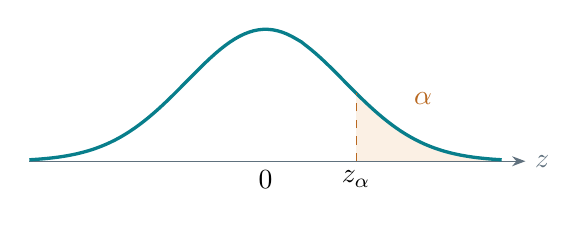
\begin{tikzpicture}[x=1.0cm,y=4.2cm,>=Stealth]
\fill[PaleAmber] (1.15,0)--plot[domain=1.15:3,samples=50](\x,{exp(-\x*\x/2)/sqrt(2*pi)})--(3,0)--cycle;
\draw[->,Muted] (-3,0)--(3.3,0) node[right] {$z$};
\draw[very thick,Teal,domain=-3:3,samples=100] plot(\x,{exp(-\x*\x/2)/sqrt(2*pi)});
\draw[dashed,Amber] (1.15,0)--(1.15,.207);
\node[below] at (1.15,0) {$z_\alpha$};\node[Amber] at (2,.19) {$\alpha$};\node[below] at (0,0) {$0$};
\end{tikzpicture}
\end{columns}
\warn{不同教材的分位数记号可能不同；以$P(Z>z_\alpha)=\alpha$这个定义为准。}
\source{笔记，第11--12页；图为上侧尾部示意。}
\end{frame}

\begin{frame}[t]{函数的分布：从$X$的取值映射到$Y=g(X)$}
\textbf{离散型：同一函数值对应的概率要合并}
\[
P(Y=y)=\sum_{x_k:g(x_k)=y}P(X=x_k).
\]
\textbf{例：}若$P(X=n)=2/3^n$，$n=1,2,\ldots$，令$Y=1+(-1)^X$。
\[
P(Y=0)=P(X\text{为奇数})=\sum_{k=0}^{\infty}\frac2{3^{2k+1}}=\frac34,
\qquad P(Y=2)=\frac14.
\]
\key{通用方法：$F_Y(y)=P\{g(X)\le y\}$。\\
先写$Y$的可能取值范围；再将不等式化为关于$X$的事件。}
\source{笔记，第12--13页；补充题-2，三、5，第4页。}
\end{frame}

\begin{frame}[t]{连续型变量变换：单调时换元，非单调时分支}
若$g$在$X$的取值区间上严格单调且可微，逆函数为$h$，在适用条件下
\[
\boxed{f_Y(y)=f_X\!\bigl(h(y)\bigr)\,|h'(y)|}.
\]
\textbf{例：}$X\sim U(-1,1)$，$Y=X^2$。此时$g$不单调，改用分布函数法：
\[
0\le y<1:\quad F_Y(y)=P(-\sqrt y\le X\le\sqrt y)=\sqrt y.
\]
\begin{columns}[T]
\column{.48\textwidth}
\[
F_Y(y)=\begin{cases}0,&y<0,\\\sqrt y,&0\le y<1,\\1,&y\ge1.\end{cases}
\]
\column{.47\textwidth}
\[
f_Y(y)=\begin{cases}\dfrac1{2\sqrt y},&0<y<1,\\0,&\text{其他}.\end{cases}
\]
\end{columns}
\source{笔记，第12--13页；平方变换为据此补充的教学例。}
\note{若只保留正根，就漏掉负半轴的一半概率。密度在0附近趋于无穷并不妨碍其积分等于1。}
\end{frame}

\begin{frame}[t]{混合型分布：连续变量经过截断可能产生点概率}
设$X\sim\Exp(\lambda)$，$\lambda>0$，令$Y=\min\{X,c\}$，$c>0$。
\begin{columns}[T]
\column{.48\textwidth}
\[
F_Y(y)=\begin{cases}0,&y<0,\\1-e^{-\lambda y},&0\le y<c,\\1,&y\ge c.\end{cases}
\]
\column{.47\textwidth}
在$y=c$处有跳跃：
\[
P(Y=c)=P(X\ge c)=e^{-\lambda c}.
\]
在$(0,c)$内仍有连续部分。
\end{columns}
\warn{只写$(0,c)$上的导数会漏掉$Y=c$的点概率；不能用普通密度完整表示这个分布。}
\source{自测题-2，二、4，第2--3页及四、8，第6--7页；参数统一为率$\lambda$。}
\end{frame}

\begin{frame}[t]{第二章收束：把题目放回“分布—概率—变换”主线}
\begin{enumerate}
\item \textbf{给分布律或密度求参数：}非负性加规范性，再使用附加条件。
\item \textbf{给$F$求概率：}检查端点是否有跳跃，保留正确的左极限。
\item \textbf{给$f$求$F$：}按非零区间分段积分，补齐区间外的0和1。
\item \textbf{求$g(X)$的分布：}先求值域；优先写$P(g(X)\le y)$。
\item \textbf{连续观测转为次数：}先算一次成功概率$p$，再判断是否为$B(n,p)$。
\end{enumerate}
\key{分布函数$F$适用于离散型、连续型和混合型，是本章最通用的工具。}
\source{根据自测题-2、补充题-2归纳。}
\end{frame}

\begin{frame}[t]{第二章练习1：分布函数中的端点与跳跃}
\begin{columns}[T]
\column{.44\textwidth}
\begin{block}{已知分布函数}
\[
F(x)=\begin{cases}0,&x<0,\\x/2,&0\le x<1,\\2/3,&1\le x<2,\\11/12,&2\le x<4,\\1,&x\ge4.\end{cases}
\]
\end{block}
\column{.51\textwidth}
\textbf{求下列概率\quad 建议4分钟}
\begin{enumerate}
\item $P(X=1)$；
\item $P(\tfrac12<X<1)$；
\item $P(2\le X\le3)$；
\item $P(X<4)$；
\item $P(X\ge2)$。
\end{enumerate}
\end{columns}
\source{自测题-2，四、1，第3--4页。}
\end{frame}

\begin{answerframe}{第二章练习1答案：有跳点时逐个处理端点}
\renewcommand{\arraystretch}{1.5}
\begin{center}
\begin{tabular}{lll}
\toprule
目标 & 分布函数表达式 & 结果\\\midrule
$P(X=1)$ & $F(1)-F(1-)=\frac23-\frac12$ & {\color{Teal}$\tfrac16$}\\
$P(\frac12<X<1)$ & $F(1-)-F(\frac12)=\frac12-\frac14$ & {\color{Teal}$\tfrac14$}\\
$P(2\le X\le3)$ & $F(3)-F(2-)=\frac{11}{12}-\frac23$ & {\color{Teal}$\tfrac14$}\\
$P(X<4)$ & $F(4-)$ & {\color{Teal}$\tfrac{11}{12}$}\\
$P(X\ge2)$ & $1-F(2-)=1-\frac23$ & {\color{Teal}$\tfrac13$}\\\bottomrule
\end{tabular}
\end{center}
\key{检查：连续部分质量为$1/2$；三个跳点质量为$1/6,1/4,1/12$，合计为1。}
\source{自测题-2，四、1，第3--4页。}
\end{answerframe}

\begin{frame}[t]{第二章练习2：正态分布与二项分布的衔接}
\begin{block}{题目\quad 建议5分钟}
某类电子元件的电阻$X$（单位：$\Omega$）服从正态分布
\[
X\sim N(50,10.4),
\]
其中第二个参数10.4为\textbf{方差}。随机检查15个元件，假定各元件电阻相互独立、同分布。

求这15个元件中\textbf{至少2个}电阻大于$55\,\Omega$的概率。
\end{block}
\textbf{提示：}先定义单个元件的“成功”事件，再定义成功元件的个数。

查表可用：$\Phi(1.55)\approx0.9394$。
\source{自测题-2，四、3，第4页；补明独立同分布假设。}
\end{frame}

\begin{answerframe}{第二章练习2答案：先算单次概率，再数成功次数}
单个元件电阻超标的概率为
\[
p=P(X>55)=1-\Phi\!\left(\frac{55-50}{\sqrt{10.4}}\right).
\]
令$Y$为15个元件中电阻大于55的个数，由独立同分布假设，
\[
Y\sim B(15,p).
\]
因此
\[
\boxed{P(Y\ge2)=1-(1-p)^{15}-15p(1-p)^{14}}.
\]
用$z\approx1.55$查表，$p\approx0.0606$，所得概率约为$\boxed{0.2296}$。
\warn{标准化除以$\sqrt{10.4}$；“至少2个”要同时扣除0个和1个。}
\source{自测题-2，四、3，第4页；末值采用题中查表精度。}
\end{answerframe}

\section{第三章\quad 二维随机变量}

\begin{frame}[t]{第三章概览：两维信息如何提取与转换}
\begin{center}
\begin{tikzpicture}[>=Stealth,
 box/.style={draw=Teal,fill=PaleTeal,rounded corners=2pt,align=center,
 minimum width=3.3cm,minimum height=1cm}]
\node[box] (j) at (0,0) {联合分布\\$F_{X,Y},\ p_{ij},\ f_{X,Y}$};
\node[box] (m) at (5,1) {边缘分布\\求和／积分消去另一变量};
\node[box] (c) at (5,-1) {条件分布\\联合除以对应边缘};
\node[box] (g) at (10,0) {函数的分布\\$Z=g(X,Y)$};
\draw[->,thick,Teal] (j)--(m);\draw[->,thick,Teal] (j)--(c);
\draw[->,thick,Teal] (j.east)--(g.west);
\end{tikzpicture}
\end{center}
\begin{itemize}
\item \textbf{离散型：}联合分布表是核心，按行、列或目标函数值求和。
\item \textbf{连续型：}先画密度非零区域，再写积分限。
\item \textbf{独立性：}满足条件时，联合分布可以分解成边缘分布的乘积。
\end{itemize}
\source{笔记，第14--22页；自测题-3与补充题-3。}
\end{frame}

\begin{frame}[t]{联合分布函数：矩形概率用“四角相减”}
\[
F(x,y)=P(X\le x,Y\le y).
\]
\begin{block}{矩形概率：$a<b$，$c<d$}
\[
\boxed{P(a<X\le b,c<Y\le d)=F(b,d)-F(a,d)-F(b,c)+F(a,c)}.
\]
\end{block}
\begin{itemize}
\item 对每个坐标单调不减、分别右连续。
\item $F(-\infty,y)=F(x,-\infty)=0$，$F(+\infty,+\infty)=1$。
\item 每个矩形的四角差都必须非负；仅坐标单调仍不够。
\end{itemize}
\key{边缘分布函数：$F_X(x)=F(x,+\infty)$，$F_Y(y)=F(+\infty,y)$。}
\source{笔记，第14--16页；补充题-3，一、7及四、3。}
\end{frame}

\begin{frame}[t]{离散型联合与边缘分布：先列清所有取值对}
袋中有编号为$-1,1,1,2$的4个球，无放回取两次，$X,Y$分别表示两次号码。
\renewcommand{\arraystretch}{1.45}
\begin{center}
\begin{tabular}{c|ccc|c}
\toprule
$Y\backslash X$ & $-1$ & $1$ & $2$ & $P(Y=y)$\\\midrule
$-1$ & $0$ & $1/6$ & $1/12$ & $1/4$\\
$1$ & $1/6$ & $1/6$ & $1/6$ & $1/2$\\
$2$ & $1/12$ & $1/6$ & $0$ & $1/4$\\\midrule
$P(X=x)$ & $1/4$ & $1/2$ & $1/4$ & $1$\\\bottomrule
\end{tabular}
\end{center}
\[
p_{ij}=P(X=x_i,Y=y_j),\quad P(X=x_i)=\sum_jp_{ij},\quad P(Y=y_j)=\sum_ip_{ij}.
\]
\source{补充题-3，四、4，第7--8页。表中两个编号为1的球仍是不同实物。}
\end{frame}

\begin{frame}[t]{连续型联合密度：概率积在“目标区域与支撑的交集”上}
\begin{columns}[T]
\column{.53\textwidth}
\[
f(x,y)\ge0,\qquad\iint_{\R^2}f(x,y)\dd x\dd y=1.
\]
若密度非零区域为$D$，则
\[
P\{(X,Y)\in G\}=\iint_{G\cap D}f(x,y)\dd x\dd y.
\]
\textbf{贯穿例：}
\[
f(x,y)=\begin{cases}k,&0<x<1,\ 0<y<2x,\\0,&\text{其他}.\end{cases}
\]
\[
1=\int_0^1\!\int_0^{2x}k\dd y\dd x=k\Rightarrow k=1.
\]
\column{.42\textwidth}
\centering
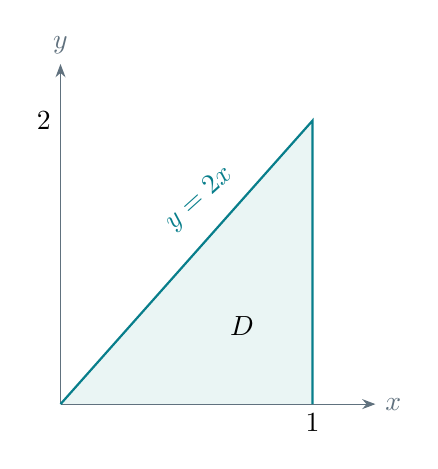
\begin{tikzpicture}[x=3.2cm,y=1.8cm,>=Stealth]
\fill[PaleTeal] (0,0)--(1,0)--(1,2)--cycle;
\draw[->,Muted] (0,0)--(1.25,0) node[right] {$x$};
\draw[->,Muted] (0,0)--(0,2.4) node[above] {$y$};
\draw[thick,Teal] (0,0)--(1,2)--(1,0);
\node[below] at (1,0) {$1$};\node[left] at (0,2) {$2$};
\node[Teal,rotate=42] at (.55,1.45) {$y=2x$};\node at (.72,.55) {$D$};
\end{tikzpicture}
\end{columns}
\source{笔记，第15--17页；自测题-3，四、2，第4--6页。}
\end{frame}

\begin{frame}[t]{边缘密度：保留谁，就对另一个变量积分}
对上页的密度$f(x,y)=\ind_{\{0<x<1,\,0<y<2x\}}$，
\begin{columns}[T]
\column{.48\textwidth}
\textbf{固定$x$，沿竖直线积分}
\[
f_X(x)=\int_{-\infty}^{\infty}f(x,y)\dd y
\]
\[
=\begin{cases}2x,&0<x<1,\\0,&\text{其他}.\end{cases}
\]
此时$y$从0到$2x$。
\column{.47\textwidth}
\textbf{固定$y$，沿水平线积分}
\[
f_Y(y)=\int_{-\infty}^{\infty}f(x,y)\dd x
\]
\[
=\begin{cases}1-y/2,&0<y<2,\\0,&\text{其他}.\end{cases}
\]
此时$x$从$y/2$到1。
\end{columns}
\key{先从图上读出切片端点；两个边缘密度各自积分都应等于1。}
\source{笔记，第16--17页；自测题-3，四、2(2)，第5页。}
\end{frame}

\begin{frame}[t]{条件分布：联合除以“条件那一边”的边缘}
\begin{columns}[T]
\column{.48\textwidth}
\begin{block}{离散型：$P(X=x_i)>0$}
\[
P(Y=y_j\mid X=x_i)=\frac{p_{ij}}{P(X=x_i)}.
\]
在前面的取球例中，
\[
P(Y=2\mid X=1)=\frac{1/6}{1/2}=\frac13.
\]
给定$X=x_i$后，沿对应列归一化。
\end{block}
\column{.47\textwidth}
\begin{block}{连续型：在$f_X(x)>0$处}
\[
f_{Y\mid X}(y\mid x)=\frac{f(x,y)}{f_X(x)}.
\]
对三角形上的贯穿例，
\[
f_{Y\mid X}(y\mid x)=\begin{cases}1/(2x),&0<y<2x,\\0,&\text{其他},\end{cases}
\]
其中$0<x<1$，即$Y\mid X=x\sim U(0,2x)$。
\end{block}
\end{columns}
\source{笔记，第17--18页；补充题-3，四、4--5；自测题-3，四、2(3)。}
\end{frame}

\begin{frame}[t]{给定$X=x$与给定$X\le x$：两种不同的条件}
仍设$f(x,y)=1$，$0<x<1$、$0<y<2x$。
\begin{columns}[T]
\column{.48\textwidth}
\begin{block}{给定一个值：用条件密度}
\[
P(Y\le\tfrac12\mid X=\tfrac12)=\int_0^{1/2}1\dd y=\boxed{\frac12}.
\]
取$x=1/2$处的切片，归一化。
\end{block}
\warn{这里通过条件密度定义，不能直接作$P(AB)/P(B)$的$0/0$运算。}
\column{.47\textwidth}
\begin{block}{给定一个事件：用概率之比}
记$A=\{Y\le1/2\}$、$B=\{X\le1/2\}$。
\[
P(A\mid B)=\frac{P(AB)}{P(B)}.
\]
\[
P(AB)=\int_0^{1/2}\!\int_{y/2}^{1/2}1\dd x\dd y=\frac3{16}.
\]
分母$\int_0^{1/2}2x\dd x=1/4$，故答案为$\boxed{3/4}$。
\end{block}
\end{columns}
\source{自测题-3，四、2(4)--(5)，第5页。}
\end{frame}

\begin{frame}[t]{随机变量独立：联合分布能否分解？}
\renewcommand{\arraystretch}{1.5}
\begin{tabular}{p{2.2cm}p{10.6cm}}
\toprule
一般情形 & 对所有$x,y$，$F(x,y)=F_X(x)F_Y(y)$\\
离散型 & 对所有$i,j$，$p_{ij}=p_{i\cdot}\,p_{\cdot j}$\\
连续型 & $f(x,y)=f_X(x)f_Y(y)$几乎处处成立\\\bottomrule
\end{tabular}
\vspace{2mm}
\begin{itemize}
\item $X,Y$独立，则适当的可测函数$g(X),h(Y)$也独立。
\item 只知道两个边缘分布，通常不能唯一确定联合分布。
\item 三角形支撑的贯穿例不独立：边缘密度的乘积在三角形外的一片区域仍为正。
\end{itemize}
\begin{block}{二维正态的特殊性质}
若$(X,Y)$服从非退化二维正态分布，则$X,Y$各自正态，且$X,Y$独立$\iff\rho=0$。
\end{block}
\source{笔记，第17--20页；自测题-3，三、2--5；补充题-3，二、3。}
\end{frame}

\begin{frame}[t]{离散型函数的分布：按相同函数值聚合概率}
\[
\boxed{P\{g(X,Y)=z\}=\sum_{(x_i,y_j):\,g(x_i,y_j)=z}p_{ij}}.
\]
回到编号$-1,1,1,2$的无放回取球例，令$S=X+Y$：
\renewcommand{\arraystretch}{1.5}
\begin{center}
\begin{tabular}{c|cccc}
\toprule
$s$ & $0$ & $1$ & $2$ & $3$\\\midrule
对应取值对 & $(-1,1),(1,-1)$ & $(-1,2),(2,-1)$ & $(1,1)$ & $(1,2),(2,1)$\\
$P(S=s)$ & $1/3$ & $1/6$ & $1/6$ & $1/3$\\\bottomrule
\end{tabular}
\end{center}
\key{“先列联合分布，再按目标值求和”适用于和、差、积、最大值、最小值。}
\source{笔记，第20页；补充题-3，四、4(3)，第8页。}
\end{frame}

\begin{frame}[t]{和的分布：一般积分公式与独立时的卷积}
对二维连续型随机变量，令$S=X+Y$，则
\[
f_S(s)=\int_{-\infty}^{\infty}f_{X,Y}(x,s-x)\dd x.
\]
\textbf{当$X,Y$独立时}，才能写成卷积
\[
\boxed{f_S(s)=\int_{-\infty}^{\infty}f_X(x)f_Y(s-x)\dd x}.
\]
\begin{columns}[T]
\column{.48\textwidth}
\textbf{例：}$X,Y$独立且均为$U(0,1)$。
\[
0<x<1,\ 0<s-x<1
\]
\[
\Longrightarrow\ \max(0,s-1)<x<\min(1,s).
\]
\column{.47\textwidth}
\[
f_S(s)=\begin{cases}s,&0<s<1,\\2-s,&1\le s<2,\\0,&\text{其他}.\end{cases}
\]
相加后是三角形密度，并非均匀分布。
\end{columns}
\source{笔记，第20--21页；自测题-3，二、2；据此补充卷积推导。}
\end{frame}

\begin{frame}[t]{正态变量的线性组合：把独立条件写在前面}
若$X\sim N(\mu_1,\sigma_1^2)$、$Y\sim N(\mu_2,\sigma_2^2)$且\textbf{相互独立}，则
\[
aX+bY+c\sim N\!\left(a\mu_1+b\mu_2+c,\ a^2\sigma_1^2+b^2\sigma_2^2\right),
\]
其中$a,b$不全为0。
\begin{block}{特别地}
\[
X+Y\sim N(\mu_1+\mu_2,\sigma_1^2+\sigma_2^2),
\]
\[
X-Y\sim N(\mu_1-\mu_2,\sigma_1^2+\sigma_2^2).
\]
\end{block}
\warn{“两个边缘分布都正态”不能推出“联合分布二维正态”，也不能单独保证其和正态。}
\source{笔记，第12、21页；自测题-3，二、1及三、2、5；补充题-3，二、6。}
\end{frame}

\begin{frame}[t]{最大值与最小值：先把不等式转成事件}
设$M=\max(X,Y)$，$N=\min(X,Y)$。
\begin{columns}[T]
\column{.48\textwidth}
\begin{block}{最大值：两者都不大于$z$}
\[
\{M\le z\}=\{X\le z,Y\le z\}.
\]
一般地$F_M(z)=F(z,z)$。
若独立，
\[
\boxed{F_M(z)=F_X(z)F_Y(z)}.
\]
\end{block}
\column{.47\textwidth}
\begin{block}{最小值：先求两者都大于$z$}
\[
\{N>z\}=\{X>z,Y>z\}.
\]
一般地$F_N(z)=F_X(z)+F_Y(z)-F(z,z)$。
若独立，
\[
\boxed{F_N(z)=1-[1-F_X(z)][1-F_Y(z)]}.
\]
\end{block}
\end{columns}
\key{最大值用“都小”；最小值的补事件用“都大”。乘积形式需要独立。}
\source{笔记，第21--22页；自测题-3，一、3及二、3--4；补充题-3，二、5。}
\end{frame}

\begin{frame}[t]{独立同分布样本的最值：由两维推广到$n$维}
若$X_1,\ldots,X_n$相互独立，具有共同分布函数$F$，则
\[
F_{\max_iX_i}(z)=F(z)^n,\qquad F_{\min_iX_i}(z)=1-[1-F(z)]^n.
\]
若共同密度为$f$，求导得到
\[
f_{\max_iX_i}(z)=nF(z)^{n-1}f(z),\qquad f_{\min_iX_i}(z)=n[1-F(z)]^{n-1}f(z).
\]
\begin{block}{例：$X_i\sim U(0,\theta)$，$\theta>0$}
在$0<z<\theta$上，
\[
f_{\max}(z)=\frac{nz^{n-1}}{\theta^n},\qquad f_{\min}(z)=\frac{n(\theta-z)^{n-1}}{\theta^n};
\]
区间外密度均为0。
\end{block}
\source{笔记，第19--22页；自测题-3，四、5，第7--8页。}
\end{frame}

\begin{frame}[t]{第三章收束：连续型综合题的固定路线}
\begin{enumerate}
\item \textbf{画支撑$D$：}写清$x,y$范围以及变量之间的不等式。
\item \textbf{规范化：}$\iint_D f(x,y)\dd x\dd y=1$求待定常数。
\item \textbf{求边缘：}固定一个变量，沿另一方向在$D$内积分。
\item \textbf{求条件：}联合密度除以条件变量的边缘密度。
\item \textbf{判独立：}比较联合与边缘乘积，或找事件概率的反例。
\item \textbf{求函数分布：}$F_Z(z)=\iint_{D\cap\{g(x,y)\le z\}}f(x,y)\dd x\dd y$。
\end{enumerate}
\key{分段点来自直线或曲线与支撑边界相交的位置；先确定分段，再积分。}
\source{自测题-3，四、2；补充题-3，四、6、9、13--14。}
\end{frame}

\begin{frame}[t]{第三章练习1：最大值、最小值的联合分布}
\begin{block}{题目\quad 建议5分钟}
$\xi,\eta$相互独立，且具有相同分布
\[
P(\xi=i)=P(\eta=i)=\frac13,\qquad i=1,2,3.
\]
令$X=\max(\xi,\eta)$，$Y=\min(\xi,\eta)$。
\begin{enumerate}
\item 求$(X,Y)$的联合分布律及两个边缘分布律。
\item 判断$X,Y$是否独立，并说明理由。
\end{enumerate}
\end{block}
\textbf{提示：}原始有序取值对共9个且等可能；$(X,Y)$必满足$X\ge Y$。
\source{自测题-3，四、1，第4页；增加独立性判断。}
\end{frame}

\begin{answerframe}{第三章练习1答案：对角线计一次，非对角线计两次}
当$x=y$时，对应$(\xi,\eta)=(x,x)$，概率为$1/9$；当$x>y$时，对应两个有序对，概率为$2/9$。
\renewcommand{\arraystretch}{1.4}
\begin{center}
\begin{tabular}{c|ccc|c}
\toprule
$Y\backslash X$ & $1$ & $2$ & $3$ & $P(Y=y)$\\\midrule
$1$ & $1/9$ & $2/9$ & $2/9$ & $5/9$\\
$2$ & $0$ & $1/9$ & $2/9$ & $3/9$\\
$3$ & $0$ & $0$ & $1/9$ & $1/9$\\\midrule
$P(X=x)$ & $1/9$ & $3/9$ & $5/9$ & $1$\\\bottomrule
\end{tabular}
\end{center}
$X,Y$\textbf{不独立}，因为
\[
P(X=1,Y=3)=0\ne P(X=1)P(Y=3)=\frac1{81}.
\]
\source{自测题-3，四、1，第4页。}
\end{answerframe}

\begin{frame}[t]{第三章练习2：三角形区域上的联合密度}
\begin{columns}[T]
\column{.59\textwidth}
\begin{block}{题目\quad 建议7分钟}
设$(X,Y)$的联合密度为
\[
f(x,y)=\begin{cases}kxy,&0<x<y<1,\\0,&\text{其他}.\end{cases}
\]
求：
\begin{enumerate}
\item 常数$k$；
\item 两个边缘密度，并判断独立性；
\item $P(X+Y>1)$；
\item $P(Y<\tfrac12\mid X<\tfrac12)$。
\end{enumerate}
\end{block}
\column{.36\textwidth}
\centering
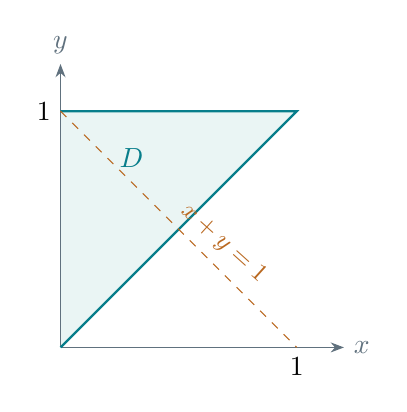
\begin{tikzpicture}[scale=3.0,>=Stealth]
\fill[PaleTeal] (0,0)--(0,1)--(1,1)--cycle;
\draw[->,Muted] (0,0)--(1.2,0) node[right] {$x$};
\draw[->,Muted] (0,0)--(0,1.2) node[above] {$y$};
\draw[thick,Teal] (0,0)--(1,1)--(0,1);
\draw[dashed,Amber] (0,1)--(1,0);
\node[below] at (1,0) {$1$};\node[left] at (0,1) {$1$};
\node[Teal] at (.3,.8) {$D$};
\node[Amber,font=\small,rotate=-42] at (.69,.44) {$x+y=1$};
\end{tikzpicture}
\end{columns}
\source{补充题-3，四、6，第9页；不改变原题密度及所求内容。}
\end{frame}

\begin{answerframe}{第三章练习2答案（1）：规范化、边缘、独立性}
\[
1=\int_0^1\!\int_0^y kxy\dd x\dd y
=\frac{k}{2}\int_0^1y^3\dd y=\frac{k}{8}\quad\Longrightarrow\quad\boxed{k=8}.
\]
\begin{columns}[T]
\column{.48\textwidth}
\[
f_X(x)=\int_x^1 8xy\dd y
\]
\[
=\begin{cases}4x(1-x^2),&0<x<1,\\0,&\text{其他}.\end{cases}
\]
\column{.47\textwidth}
\[
f_Y(y)=\int_0^y8xy\dd x
\]
\[
=\begin{cases}4y^3,&0<y<1,\\0,&\text{其他}.\end{cases}
\]
\end{columns}
$X,Y$\textbf{不独立}：$P(X>1/2,Y<1/2)=0$，而两个边缘事件的概率均大于0。
\source{补充题-3，四、6，第9页。}
\end{answerframe}

\begin{answerframe}{第三章练习2答案（2）：画交集，条件事件作分母}
\textbf{（3）}在$0<x<y<1$中加入$x+y>1$，得到$1/2<y<1$、$1-y<x<y$：
\[
P(X+Y>1)=\int_{1/2}^1\!\int_{1-y}^y8xy\dd x\dd y
=\int_{1/2}^1 4y(2y-1)\dd y=\boxed{\frac56}.
\]
\textbf{（4）}由于$X<Y$，事件$\{Y<1/2\}$包含在$\{X<1/2\}$中，故
\[
P(Y<\tfrac12\mid X<\tfrac12)=\frac{P(Y<1/2)}{P(X<1/2)}
=\frac{\int_0^{1/2}4y^3\dd y}{\int_0^{1/2}4x(1-x^2)\dd x}
=\frac{1/16}{7/16}=\boxed{\frac17}.
\]
\key{先利用事件的包含关系化简，再积分，可以减少计算量。}
\source{补充题-3，四、6，第9页。}
\end{answerframe}

\section{全课回顾}
\begin{frame}[t]{把三章连起来：始终在求某个事件的概率}
\renewcommand{\arraystretch}{1.6}
\begin{tabular}{p{3cm}p{9.7cm}}
\toprule
\textbf{描述方式} & \textbf{基本计算}\\\midrule
事件概率 & $P(A\mid B)=P(AB)/P(B)$；用划分拆解复杂事件\\
一维分布律 & $P(X\in A)=\sum_{x_k\in A}p_k$\\
一维密度 & $P(X\in A)=\int_Af_X(x)\dd x$\\
二维联合密度 & $P((X,Y)\in G)=\iint_Gf(x,y)\dd x\dd y$\\
函数的分布 & $F_Z(z)=P(g(X,Y)\le z)$；一维情形同理\\\bottomrule
\end{tabular}
\key{事件运算负责“把目标写对”，分布负责“把概率算出”。}
\source{根据第1--3章笔记及六份习题归纳。}
\end{frame}

\begin{frame}[t]{课后自查：六个高频失分点}
\begin{enumerate}
\item 把$P(A\mid B)$与$P(B\mid A)$互换。
\item 未检查独立性，就把交事件概率写成乘积。
\item 在分布函数有跳跃时，忽略端点开闭。
\item 把密度值$f(x)$当作点概率$P(X=x)$。
\item 二重积分只看目标事件，遗漏密度的非零区域。
\item 求变换后的分布时，漏写值域、分段或点概率。
\end{enumerate}
\key{做完一道题，至少检查：\textbf{条件齐全、范围正确、总概率为1}。}
\source{根据六份习题中的判断题、选择题与综合题归纳。}
\end{frame}

\appendix
\section{选讲附录}
\begin{frame}[t]{附录A：二维正态分布的密度与边缘}
非退化二维正态分布记为
$(X,Y)\sim N_2(\mu_1,\mu_2,\sigma_1^2,\sigma_2^2,\rho)$，其中$\sigma_1,\sigma_2>0$、$|\rho|<1$。
令$u=(x-\mu_1)/\sigma_1$，$v=(y-\mu_2)/\sigma_2$，其联合密度为
\[
f(x,y)=\frac1{2\pi\sigma_1\sigma_2\sqrt{1-\rho^2}}
\exp\!\left\{-\frac{u^2-2\rho uv+v^2}{2(1-\rho^2)}\right\}.
\]
\begin{itemize}
\item 边缘分布：$X\sim N(\mu_1,\sigma_1^2)$，$Y\sim N(\mu_2,\sigma_2^2)$。
\item 在二维正态前提下，$\rho=0$等价于独立。
\item 联合正态保证线性组合仍为正态；两个边缘正态不能代替这一前提。
\end{itemize}
\source{笔记，第17、19页；自测题-3，三、2及5。此页为选讲。}
\end{frame}

\begin{frame}[t]{附录B：乘积与商的密度公式}
若$(X,Y)$有联合密度$f_{X,Y}$，在适用条件下：\par
\textbf{乘积$Z=XY$}
\[
\boxed{f_Z(z)=\int_{-\infty}^{\infty}\frac1{|x|}f_{X,Y}\!\left(x,\frac z x\right)\dd x}.
\]
\textbf{商$W=X/Y$}
\[
\boxed{f_W(w)=\int_{-\infty}^{\infty}|y|f_{X,Y}(wy,y)\dd y}.
\]
\warn{必须由原支撑确定积分限；独立时可把联合密度换成边缘乘积。绝对值因子不能遗漏。}
\source{笔记，第21页乘积与商的分布；公式按统一符号重写。此页为选讲。}
\end{frame}

\begin{frame}[t]{附录C：多维推广，仍然是消元与分解}
\textbf{联合分布函数}
\[
F(x_1,\ldots,x_n)=P(X_1\le x_1,\ldots,X_n\le x_n).
\]
\textbf{边缘密度：}把不需要的变量全部积分掉，例如
\[
f_{X_1}(x_1)=\int_{\R^{n-1}}f(x_1,x_2,\ldots,x_n)\dd x_2\cdots\dd x_n.
\]
\textbf{相互独立：}对所有$x_1,\ldots,x_n$，
\[
F(x_1,\ldots,x_n)=\prod_{i=1}^nF_{X_i}(x_i).
\]
\key{若两个随机向量相互独立，则分别由它们构造的可测函数也相互独立。}
\source{笔记，第19--20页。此页为选讲。}
\end{frame}

\begin{frame}[t]{附录D：概率积分变换，连接分布函数与均匀分布}
若$X$的分布函数$F_X$连续，则
\[
\boxed{U=F_X(X)\sim U(0,1)}.
\]
进一步令$Z=-2\ln U$。当$z\ge0$时，
\[
F_Z(z)=P(-2\ln U\le z)=P(U\ge e^{-z/2})=1-e^{-z/2}.
\]
于是
\[
f_Z(z)=\begin{cases}\dfrac12e^{-z/2},&z>0,\\0,&\text{其他},\end{cases}
\qquad Z\sim\Exp(1/2).
\]
\warn{$F_X$连续不代表处处严格递增；不能未经检查就直接假设普通反函数存在。}
\source{自测题-2，四、6，第5--6页；补全原解析中反函数使用的条件提醒。此页为选讲。}
\end{frame}

\end{document}
